%-----------------------------------------------------------------------------
%
%               Template for sigplanconf LaTeX Class
%
% Name:         sigplanconf-template.tex
%
% Purpose:      A template for sigplanconf.cls, which is a LaTeX 2e class
%               file for SIGPLAN conference proceedings.
%
% Guide:        Refer to "Author's Guide to the ACM SIGPLAN Class,"
%               sigplanconf-guide.pdf
%
% Author:       Paul C. Anagnostopoulos
%               Windfall Software
%               978 371-2316
%               paul@windfall.com
%
% Created:      15 February 2005
%
%-----------------------------------------------------------------------------


\documentclass[preprint, numbers]{sigplanconf}

% The following \documentclass options may be useful:

% preprint       Remove this option only once the paper is in final form.
%  9pt           Set paper in  9-point type (instead of default 10-point)
% 11pt           Set paper in 11-point type (instead of default 10-point).
% numbers        Produce numeric citations with natbib (instead of default author/year).
% authorversion  Prepare an author version, with appropriate copyright-space text.

%\usepackage[para]{footmisc}

\usepackage{natbib,hyperref}
\usepackage{url}
\usepackage{verbatim}
\usepackage{graphicx}

\newcommand{\cL}{{\cal L}}

\begin{document}

\special{papersize=8.5in,11in}
\setlength{\pdfpageheight}{\paperheight}
\setlength{\pdfpagewidth}{\paperwidth}

\conferenceinfo{CONF'yy}{Month d--d, 20yy, City, ST, Country}
\copyrightyear{20yy}
\copyrightdata{978-1-nnnn-nnnn-n/yy/mm}\reprintprice{\$15.00}
\copyrightdoi{nnnnnnn.nnnnnnn}

% For compatibility with auto-generated ACM eRights management
% instructions, the following alternate commands are also supported.
%\CopyrightYear{2016}
%\conferenceinfo{CONF'yy,}{Month d--d, 20yy, City, ST, Country}
%\isbn{978-1-nnnn-nnnn-n/yy/mm}\acmPrice{\$15.00}
%\doi{http://dx.doi.org/10.1145/nnnnnnn.nnnnnnn}

% Uncomment the publication rights used.
%\setcopyright{acmcopyright}
\setcopyright{acmlicensed}  % default
%\setcopyright{rightsretained}

%\titlebanner{banner above paper title}        % These are ignored unless
\preprintfooter{Continuations Code Reviews on any code inside the IDE}   % 'preprint' option specified.

\title{Continous Peer Reviews}
\subtitle{A Social Coding tool for Code Reviews inside the IDE}

\authorinfo{Tobias D{\"u}rschmid}
           {Hasso Plattner Institute}
           {tobias.duerschmid@student.hpi.de}

\maketitle

\begin{abstract}
Code reviews play an important and successful role in modern software development. 
%
But usually they happen only once before new code is merged into the main branch.
%
We preset a concept that helps developers to continuously give feedback on their source code directly in the IDE by using the metaphor of social networks. 
%
This reduces context switches for developers, improves the software develop process and allows to give feedback to developers of external libraries and frameworks. 
\end{abstract}

% 2012 ACM Computing Classification System (CSS) concepts
% Generate at 'http://dl.acm.org/ccs/ccs.cfm'.
\begin{CCSXML}<ccs2012>
<concept>
<concept_id>10003120.10003130.10003233</concept_id>
<concept_desc>Human-centered computing~Collaborative and social computing systems and tools</concept_desc>
<concept_significance>500</concept_significance>
</concept>
<concept>
<concept_id>10011007.10011006.10011066.10011069</concept_id>
<concept_desc>Software and its engineering~Integrated and visual development environments</concept_desc>
<concept_significance>300</concept_significance>
</concept>
<concept>
<concept_id>10011007.10011074.10011134</concept_id>
<concept_desc>Software and its engineering~Collaboration in software development</concept_desc>
<concept_significance>100</concept_significance>
</concept>
</ccs2012>
\end{CCSXML}

\ccsdesc[500]{Human-centered computing~Collaborative and social computing systems and tools}
\\
\ccsdesc[300]{Software and its engineering~Integrated and visual development environments}
\ccsdesc[100]{Software and its engineering~Collaboration in software development}
% end generated code

% Legacy 1998 ACM Computing Classification System categories are also
% supported, but not recommended.
%\category{CR-number}{subcategory}{third-level}[fourth-level]
%\category{D.3.0}{Programming Languages}{General}
%\category{F.3.2}{Logics and Meanings of Programs}{Semantics of Programming Languages}[Program analysis]

\keywords
code review, code quality, social coding, feedback

\section{Introduction}
%\section{Problem and Motivation}
Performing code reviews is an important practice at professional companies and open source projects~\cite{balachandran2013PeerCodeReviews, bird2015CodeReviewPlatform, rigby2013PeerCodeReviews, czerwonka2015codereviews}, because developers want to finde defects, improve the code quality, dicuss alternative solutions, transfer knowledge, and improve the team awareness~\cite{rigby2013PeerCodeReviews, bacchelli2013expectations}.
%
Recent studies confirmed, that review coverage and review participation have a significant impact on code quality and the correctness of software~\cite{mcintosh2014impact, thongtanunam2015CodeReviews, shimagaki2016CRInSony}. 
%

%
But traditionally code reviews are done only once before the code is merged into the main branch~\cite{rigby2013PeerCodeReviews}. 
%
This process does not continuously give feedback on code quality (especially of legacy code), does not support questions of new developers concerning existing code and forces the developers to leave their IDE for commenting on code.
%

%
The main contribution is a new concept targeting these problems by supporting a community model for source code inside the IDE using the metaphor of social networks.
%
It allows developers to casually add comments to packages, classes, methods and method snippets with minimum effort.
%

%
Social networks like Facebook\footnote{\url{https://facebook.com}}, Twitter\footnote{\url{https://twitter.com}}, or Stack Overflow\footnote{\url{https://stackoverflow.com}} allow to comment on any contend and show happiness about the contend using an "I like" button.
% 
We transfer this metaphor to programming by offering developers to comment on any code and to like code snippets in the project using their IDE.  
%
Code reviews of large changes (20 files or more) are less useful~\cite{czerwonka2015codereviews}.
%
Therefore our approach tries to continuously give feedback just while reading a piece of code inside the IDE. 
%
Figure~\ref{overview} gives an overview over the comment model used in our tool.

\section{Background}
\subsection{Code Review}
A code review is a systematic examination of source code. 
%
Reviews forms range from very informal (e.g. pair programming~\cite{beck2000extreme}) to very formal (e.g. software inspections~\cite{fagan2001design, ackerman1989software}). 
%
Convergent peer reviews are predominantly lightweight, flexible processes, that happen early, quickly and frequently~\cite{rigby2013PeerCodeReviews, shimagaki2016CRInSony}. 
%
Therefore we refer to code reviews as informal peer reviews. 
%
 
%
Currently the main activity of reviews changes from defect finding to discussions about alternative solutions and long-term code maintainability~\cite{rigby2013PeerCodeReviews, czerwonka2015codereviews}. 
%
Only about 15\% of the peer review comments point out possible defect while 50\% address code quality~\cite{czerwonka2015codereviews}
%

%
One challenge developers are facing during code reviews is context switching, because they have to understand another issue and stop doing thier current work~\cite{czerwonka2015codereviews, kononenko2016codereviewquality}.
%
Switching from one problem space to another reduces developers productivity and should be avoided~\cite{poppendieck2003lean}.
\subsection{Social Coding}
Social coding is the community-based development of software.
%
Social coding sites like GitHub\footnote{\url{https://github.com}} and BitBucket\footnote{\url{https://bitbucket.org}} enable substantially more collaborations among developers \cite{thung2013github} and shift the focus of interaction to individual contributors and their activities with electronic artifacts~\cite{dabbish2012social}.
%
Therefore social coding is a new and promising approach for improving the software development process by encouraging the collaborations in the team.

\begin{figure}[t!]
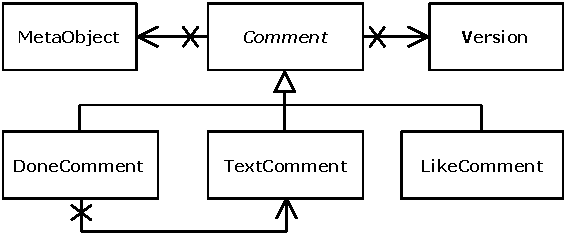
\includegraphics[width=\columnwidth]{images/Overview.pdf}
\caption{Overview over the comment model. Each comment references a meta object (e.g. class, method, package) and references a version encoding the state on which it was commented. A comment can consist of textual feedback or a like action or a done action referencing the comment that should be archived.}
\label{overview}
\end{figure}
\section{Walkthrough}
The developer Alice reads a piece of code relevant to her current issue.
%
She does not understand, why this is done like it is and just adds a comment on this piece of code. 
%
Because Bob did the last change to this code, he gets an email informing him about the new comment. 
%
He opens the concerned method and answers the questions. 
%
Alice recommends Bob to refactor the code to directly reveal this intention.
%
He does so and pushes the done button of the comment in order to hide the comment of the discussion. 
%
After Alice has finished her issue, Bob enjoys reading her code and therefore pushes the "I like" button of the new method in order to help new developer getting to know the coding styles of the project. 

\section{Related Work}
Many projects working with feature branches perform code reviews during pull requests before merging the changes into the main branch~\cite{driessen2010successful, calefato2015PLE, yu2015pullrequests, tsay2014contributionGithub, gousios2014PullBasedSD, rahman2014pullrequests, tsay2014ContributionDiscussion}. 
%
Tools like CodeFlow~\cite{bird2015CodeReviewPlatform}, Mondrian~\cite{kennedy2006Mondrian}, Gerrit~\cite{google2016gerrit},  Phabricator~\cite{tsotsis2011Phabricator} and ClusterChanges~\cite{barnett2015helpingdevelopers} support these change-based code reviews.
%
In contrast to that, our concept gives feedback on the current state of code. 
%
The reviews supported by these tools are made using a push model, meaning that developer request reviews, while our tool uses a pull model, meaning that developers can comment on any code.
%
Hence our concept allows to comment on library code and framework code and therefore give feedback to the developers of third party software. 
%
Furthermore our feedback is continuous and therefore allows new developers to comment on old code. 
%
In contrast to existing tools, our concept allows the developers to stay inside their IDE and avoid context switches. 
%
This provides a more self-sustaining environment that supports the liveness of the development process. 
%
However a dedicated review process before merging changes into the main branch let the developers focus on issues raised up by the specific changes. 
%
Therefore we propose to use our concept in conjunction with pull requests or	 other change-based reviews and not instead of it.
%
\\

%
\begin{comment}

\section*{Acknowledgment}
I would like to thank Patrick Rein for his support and the HPI software architecture group for the continous feedback.

\end{comment}

\bibliographystyle{plainnat}
\bibliography{bibliography}

\end{document}

